\chapter{Návrh uživatelského rozhraní}
\begin{chapterabstract}
    Tato kapitola pojednává o návrhu uživatelského rozhraní pro aplikaci. Nejprve bude uvedeno, proč je pro nás uživatelské rozhraní důležité a jaké jsou naše cíle při jeho návrhu. Následně budou uvedeny pojmy se kterými kapitola pracuje. Nakonec na základě požadavků vydefinovaných v předchozí kapitole budou předvedeny jednotlivé návrhy uživatelského rozhraní pro různé části aplikace, u kterých bude vysvětleno proč jsou takto navrženy, popřípadě komentář od potenciálních uživatelů, kteří se k návrhům vyjádřili.
\end{chapterabstract}

Uživatelské rozhraní je v našem případě velmi důležité, protože pokud chceme aby aplikace byla úspěšná, je potřeba aby jí do budoucna využívalo co nejvíce lidí. Proto je potřeba aby bylo uživatelské rozhraní jednoduché, přehledné a intuitivní. Zároveň ale chci dosáhnout toho, aby bylo líbivé a uživatelé bavilo se v něm pohybovat a používat ho.

\section{Wireframing}
Je to způsob, jak navrhovat uživatelské rozhraní na úrovni jeho struktury a rozložení. Wireframe je návrh layoutu stránky, který demonstruje které prvky stránka bude mít. Jeho cílem je přiblížit celému týmu a stakoholderům jak bude vypadat výsledný produkt ještě předtím, než se začne s jeho vývojem. Díky tomu se dá předejít zbytečným změnám v pozdějších fázích vývoje, které bývají nákladné. Wireframy se dají budˇvytvářet ručně, nebo pomocí různých nástrojů jako je například Figma, Adobe XD, Sketch a další. \cite{wireframing:definition}

Wireframy se dělí na tři kategorie:
\begin{itemize}
    \item Low-fidelity wireframe - jsou jednoduché, často černobílé, bez detailů a zaměřují se na především na rozložení prvků na stránce a navigaci mezi nimi. 
    \item Mid-fidelity wireframe - jsou podrobnější než low-fidelity, slouží k zpřesnění výsledného designu. Designéři do nich přidávají poznámky a konkrétnější obsah, testují různé varianty uživatelských toků a prvků rozhraní.
    \item High-fidelity wireframe - se už podobají raným verzím finálního produktu. Obsahují vizuální i interaktivní prvky, ale stále nemusí mít plnou funkčnost prototypu. \cite{wireframing:types}
\end{itemize}

V rámci projektu budu jednotlivé typy wireframů využívat podle aktuální potřeby. Jelikož však na projektu pracuji sama a nemám k dispozici UX designéra, zaměřím se především na low-fidelity a mid-fidelity wireframy, které mi umožní efektivně navrhnout strukturu a rozložení aplikace. Tvorba high-fidelity wireframů je podle mých zkušeností časově náročná, což při omezeném časovém rámci projektu není příliš vhodné.

\subsection{Figma}
Pro návrh uživatelského rozhraní jsem zvolila nástroj Figma. Figma je nástroj, který je v základní verzi zdarma a i v ní umožňuje nejenom jednoduše tvořit návrhy uživatelského rozhraní, ale také obsahuje řadu užitečných funkcionalit, které usnadnují jejich tvorbu (možnost přidávat komentáře, tvořit komponenty, prototypovat a mnoho dalšího). Já osobně mám ráda, že můžu vytvořit parent komponentu (například navigační menu) a následně její kopie vkládat na všechny stránky, které ji potřebují. Díky tomu, že jsou všechny tyto kopie propojené s parent komponentou, stačí upravit pouze parent komponentu a všechny její kopie se automaticky aktualizují. To je velmi užitečné, protože se dá ušetřit spousta času a zároveň se dá předejít chybám, které by mohly vzniknout při ruční úpravě každé kopie zvlášť. Dále se mi velmi dobře pracuje s tzv. auto layoutem, který umožňuje nastavit pravidla pro rozložení prvků na stránce, a díky tomu se dá snadno přizpůsobit návrh různým velikostem obrazovky. \cite{figma}

Navíc pro Figmu bývají již vytvořené tzv. UI kit, což jsou předpřipravené komponenty, které odpovídají určitým designovým systémům (například Material Design od Google). Díky tomu se design dá více přiblížit finálnímu vzhledu a zároveň se dá ušetřit spousta času, protože není potřeba tvořit komponenty od začátku, ale skládat je z již předpřipravených. \cite{figma:uiKits}

Tyto důvody potvrdily, že Figma je pro mě ideálním nástrojem pro návrh uživatelského rozhraní pro tento projekt. Díky zkušenostem s tímto nástrojem jsem schopná efektivně navrhnout uživatelské rozhraní.

\section{Design systém}
Design systém je soubor pravidel a opakovaně použitelných prvků, které zajišťují jednotný vzhled i celkový dojem z produktu a uživatelského prostředí. Design systém tvoří například barvy zvolené pro produkty, ikonky co budou použity, typografie, ale také způsob jakým budou fungovat interakce s uživatelem. Design systém nám pomáhá udržovat konzistentní vzhled a chování napříč různými částmi produktu, což zlepšuje uživatelský zážitek a usnadňuje orientaci v aplikaci. \cite{designSystems}

V následujících sekcích rozeberu jednotlivé knihovny s komponentami, které se dají využít jako design systém nebo minimálně základ pro vytvoření vlastního design systému.
Jelikož jsem v předchozí kapitole zvolili jako technologii pro vývoj aplikace React, zaměřím se na knihovny, které jsou určeny pro tento framework. 

\subsection{Material UI}
Material UI je knihovna implementující Material Design od Google pro React. tato knihovna obsahuje velké množství předpřipravených komponent, které jsou navrženy tak, aby odpovídaly designovým principům Material Designu. Díky tomu se dá snadno vytvořit konzistentní a moderní uživatelské rozhraní. Knihovna je velmi rozšířená a má velkou komunitu, včetně přehledné dokumentace, což usnadňuje její používání. Mezi její nevýhody patří avšak to, že knihovna má velký bundle size, což může negativně ovlivnit výkon aplikace, a také to, že má svůj specifický vzhled, který nemusí být vhodný pro všechny typy aplikací. Já osobně mám s Material UI hodně zkušeností, protože jsem s ní pracovala na bakalářské práci, a vím jak funguje. Podle mého pozorování nabízí nejvíce předpřipravených komponent, které jsou funkční a dobře se s nimi pracuji. Avšak jsem tuto knihovnu zavrhla, protože se snažím vytvořit aplikaci s poutavějším designem a snažit se ohýbat Material UI není vhodné dle mého názoru, protože to nepůjde jednodušše a zároveň tím ztrácíme částečně smysl, proč chceme použít tento design system. \cite{reactUILibraries}

\subsection{Ant Design}
Je design systém a knihovna komponent pro React, který se zaměřuje především na enterprise aplikace. Komponenty v Ant Design jsou navrženy pro firemní aplikaci (jako administrační aplikace, dashboardy a podobně), než pro aplikace, které by měly pracovat s koncovými uživateli.
Vzhledem k tomu, že vzhled komponent této knihovny se mi nelíbí a navíc se mi zdá, že je zaměřená spíše na jiné typy aplikací, než jakou chci vytvořit, jsem se rozhodla tuto knihovnu také nezvolit. \cite{reactUILibraries}

\subsection{Chakra UI}
Je další kvalitní knihovna komponent pro React, která se zaměřuje na jednoduchost a přizpůsobitelnost. Chakra UI nabízí širokou škálu komponent včetně grafů. API této knihovny je intuitivní a umožňuje snadno přizpůsobit vzhled a chování komponent. Knihovna má také skvělou dokumentaci, ve které jsou uvedeny příklady použití a možnosti přizpůsobení. Co mi však vadí na této knihovně je to, že její vzhled se mi tolik nelíbí a narazila jsem tam u některých komponent na jiné chování než bych chtěla, například u comboboxu se možnosti zakliknuté přidávají nad ním, což mi připadá nepřehledné. Díky tomuto faktu jsem se rozhodla tuto knihovnu nezvolit. \cite{reactUILibraries}

\subsection{Shadcn UI}
Shadcn UI není knihovnou design systému, ale spíše sbírkou komponent pro React, které jsou navrženy tak, aby byly co nejvíce přizpůsobitelné a umožňovaly vytvářet vlastní design systém.\cite{reactUILibraries}

Tato knihovna bývá používáná s Tailwind CSS, což je utility-first CSS framework, který umožňuje rychle a efektivně vytvářet vlastní designy. \cite{tailwindcss}

Shadcn UI samotná stojí na na Radix UI a Base UI knihovnách a dostylizovaná pomocí Tailwind CSS. Knihovna se do aplikace nestahuje jako celek, ale jednotlivé komponenty se stáhnou jako kód do projektu, což umožňuje v případě potřeby upravit komponentu přímo v projektu. Díky tomu se dá design skoro až bych řekla maximálně přizpůpsobit. Mě osobně se knihovna líbí i nastylovaná v defaultním stavu, ale zároveň ocením možnost pohrát si s designem a přizpůsobit ho podle svých představ. Díky tomu jsem se rozhodla tuto knihovnu zvolit pro tvorbu uživatelského rozhraní pro tento projekt. \cite{reactUILibraries}

\section{Tmavý režim}
Při implementaci jednotlivých komponent budu zároveň implementovat i verzi pro tmavý režim na základě požadavku TODO. Tmavý režim nenavrhuji jako samostatný design, ale spíše jako variantu světlého režimu. Ve figmě komponenty navrhuji jen ve světlém režimu, protože na návrh tmavého režimu bych musela vynaložit moc času.

\section{Theme aplikace}
Shadcn UI umožňuje nastavit globální theme pro celou aplikaci, což nám umožní definovat například barvy, které se budou používat v celé aplikaci. Díky tomu můžeme zajistit konzistentní vzhled napříč různými částmi aplikace a zároveň nám to usnadní přizpůsobení designu v budoucnu, protože pokud budeme chtít změnit například hlavní barvu aplikace, stačí upravit pouze tuto jednu hodnotu v theme a všechny komponenty, které tuto barvu používají, se automaticky aktualizují. Pro tento projekt jsem se rozhodla nastavit theme Red, protože mi přijde, že se nejvíce hodí k tanečnímu tématu oproti jiným variantám.

\section{Návrh jednotlivých částí aplikace}
V této sekci chci navrhnout jednotlivé části aplikace. U většiny částí bude přiložen návrh uživatelského rozhraní ať už pomocí wireframu, nebo přímo implementace v projektu.  

\subsection{Navigační prvky}
Nejprve je potřeba navrhnout navigační prvky, které se budou nacházet na každé stránce aplikace. Jedním z těcto prvků je navigační lišta umístěná v horní části obrazovky, která bude obsahovat název aplikace s logem a dále následující odkazy/akce:
\begin{itemize}
    \item sekci Events, která po rozkliknutí nabídne odkazy i s vysvětlením, co daná stránka obsahuje (All events - seznam nadcházejících akcí, My events - seznam akcí, na které se uživatel přihlásil, organizoval anebo označil že má zájem, Create event - formulář pro vytvoření nové akce)
    \item About, která po rozkliknutí uživatele přesměruje na stránku s informacemi o aplikaci
    \item ikonu slunce/měsíce, která bude sloužit pro přepínání mezi světlým a tmavým režimem
    \item pokud je uživatel přihlášený, bude se zde nacházet také ikona profilu, která po rozkliknutí zobrazí informace kdo je přihlášený (jméno uživatele a email) a nabídne odkazy na profil uživatele a odhlášení z aplikace
    \item pokud uživatel není přihlášený, bude se zde nacházet odkaz pro přihlášení do aplikace
\end{itemize}

Pokud jsme na stránce pro přihlášení do aplikace, navigační lišta bude obsahovat pouze název aplikace s logem.
U mobilního zobrazení bude navigační lišta obsahovat pouze název aplikace s logem, přepínač na tmavý režim a ikonu pro otevření menu, které bude obsahovat odkazy/akce jako v desktopovém zobrazení. Navigační lištu jsem implementovala rovnou v kódu, protože poskládání a prototypování v nástroji Figma by mi zabralo zbytečně moc času. Finální design navigační lišty je znázorněn na obrázku \ref{fig:navbar}.

Dále jsem navrhla pro hezčí design patičku, která se bude nacházet v dolní části obrazovky a bude obsahovat pouze název aplikace s logem.

\begin{figure}
    \centering
    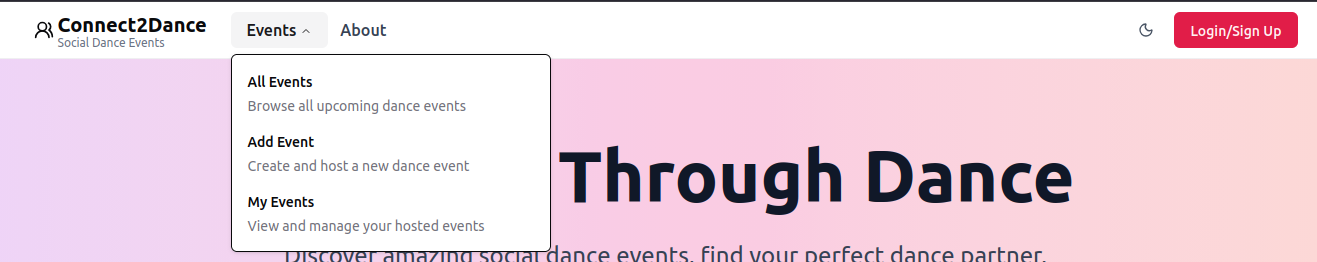
\includegraphics[width=\textwidth]{images/navbar.png}
    \caption{Finální design navigační lišty aplikace}
    \label{fig:navbar}
\end{figure}

\subsection{Domovská stránka}
Domovská stránka bude propagovat celou aplikaci a její hlavní funkce. Bude obsahovat krátký popis toho, co aplikace umí a jaké jsou její hlavní funkce. U nich budou 2 tlačítka, jedno (výraznější) pro přihlášení do aplikace a druhé pro zobrazení nadcházejících akcí. Dále bude obsahovat sekci s top funkcionalitama aplikace, proč by uživatelé měli aplikaci používat. Nakonec se zde budou nacházet 3 akce, které se konají v nejbližší době. Tento návrh jsem tvořila na základě požadavku.

Návrh domovské stránky je znázorněn na obrázku TODO.

% \begin{figure}
%     \centering
%     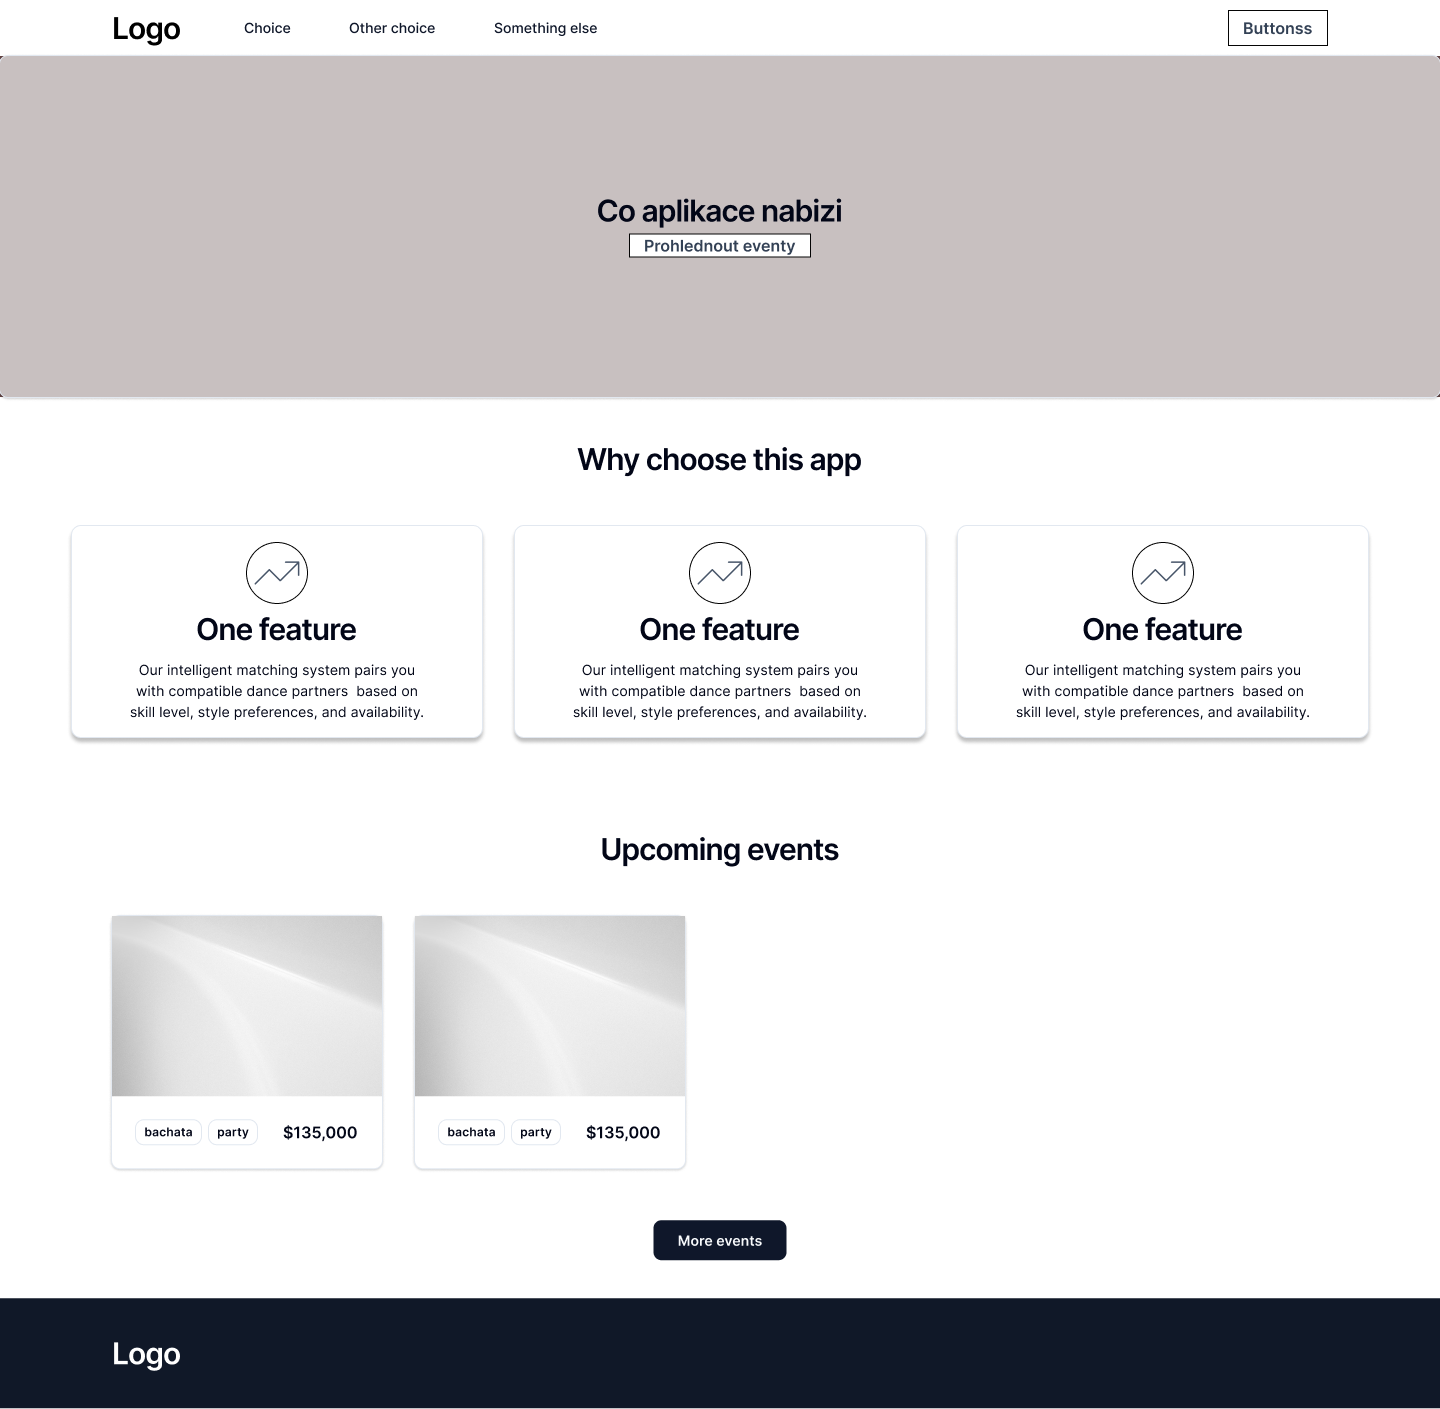
\includegraphics[width=\textwidth]{images/homePage.png}
%     \caption{Návrh domovské stránky}
%     \label{fig:homePage}
% \end{figure}

\subsection{Nadcházející akce}
Tato stránka je velmi důležitá, protože hned po úvodní stránce, je stránkou, kterou uživatelé uvidí a budou se například rozhodovat zda se zaregistrují do aplikace.

Stránka se skládá ze sekce pro vyhledávání akcí a výčtu nadcházejících akcí. Pro vyhledávání jsem navrhla několik inputů, které umožní uživatelům filtrovat akce podle různých kritérií dle požadavku TODO. 

Pro filtrování jména akce jsem se rozhodla navrhnout dlouhý input, následně pro místo konání akce jsem navrhla combobox, který umožní uživatelům potom co začnou psát název místa, zobrazit možnosti, které odpovídají zadanému textu. 

Pro typ akce a typ tance jsem navrhla také comboboxy avšak uživatel může vybrat více možností a pokud je tech možností více než tři tak se zobrazí pouze první tři a zbytek bude zobrazen jako "+X", kde X bude počet zbývajících možností. Po rozkliknutí komboboxu se uživateli zobrazí možnosti které zaškrtl. Tento výběr možností bude na mobilním zařízení implementován tak že vyjede nabídka (podobající se modalu) s možnostmi, které může uživatel zaškrtnout/odškrtnout.

Co se týče zobrazení nadcházejících akcí, navrhla jsem zobrazení ve formě karet, které budou obsahovat informace, jak jsou definované v požadavku TODO. Kartu na desktopovém zařízení jsem pojala tak, že v levé části karty se bude nacházet obrázek akce anebo placeholder pokud obrázek není uvedený. Úplně nahoře v pravé části karty bude název akce, pod ním bude jméno organizátora a následně se budou nacházet zbylé informace o akci, obohacené o ikony. Úplně na spodu karty se budou nacházet akce, když je akce organizována uživatelem, bude se zde nacházet tlačítko přejít na detail akce, pokud uživatel organizátorem není, tak zde navíc budou akce jako přihlásit se na akci a označit že mám zájem o akci. Co mi chvíli dalo zabrat na návrhu bylo umístění tagů, které budou zobrazovat typ akce a typ tance. Nakonec jsem se rozhodla umístit je pod organizátora, kvůli tomu že jsem proiterovala několik variant a tato varianta se uživatelům zdála nejpřehlednější. 

V mobilní variantě se obrázek a informace zobrazí nad sebou, aby se lépe přizpůsobily menší obrazovce.

Základ jsem si nakreslila do figmy, jak mobilní zařízení, tak desktopové zobrazení, ale finální design jsem implementovala rovnou v kódu, protože mi to přišlo efektivnější. Finální design této stránky je znázorněn na obrázku TODO.

\subsection{Detail akce}
Tahle sekce byla pro mě nejtěžší na návrh, protože se zde nachází poměrně hodně informací a akcí, které je potřeba nějak přehledně uspořádat. Při návrhu jsem vycházela z požadavku TODO a také z diskuzí s potenciálními uživateli, kteří mi poskytli cennou zpětnou vazbu ohledně toho, jaké informace by měly být zobrazeny a jak by měly být uspořádány. Při návrhu jsem se inspirovala ze stránech na pořádání událostí jak AllEvents, Eventbrite, Meetup a také z Facebooku, kde se tanečníci nejvíce dozvídají o nadcházejících akcích. Na návrhu této stránky jsem chtěla investovat více času, protože se jedná o jednu z nejklíčovějších stránek celé aplikace a díky této stránce se uživatelé rozhodují, zda se na akci přihlásí, nebo ne. 

Jako první co bude na stránce bude promo obrázek akce, který bude zobrazený v celé šířce stránky. Pokud akce nemá promo obrázek, tak se zobrazí placeholder barva. Na tomto obrázku dole se bude nacházet název akce a pod ním klíčové informace o akci (tyto informace jsou sepsané v požadavku TODO jako základní informace o akci). 

Potom stránka bude obsahovat tlačítka, která umožní pracovat s touto událostí. Tlačítka se liší podle toho zda je uživatel organizátorem akce, přihlášeným uživatelem, nebo uživatelem, který není přihlášený na akci. Pozici tlačítek jsem umístila pod promo obrázek s informacemi o akci, aby byli co nejvíce dostupné a nabádali uživatele k akci. Pokud je uživatel organizátorem akce, bude se zde nacházet tlačítko pro správu akce, které po rozkliknutí nabídne možnosti jako upravit akci a dále podle toho v jakém je akce stavu (smazat/zrušit, publikovat). Pokud uživatel organizátorem není, tak se zobrazují tlačítko pro přihlášení na akci a označení že mám zájem o akci.  

Následně se budou nacházet na stránce tyto sekce (seřazeny od nejdůležitější po nejméně důležitou):
\begin{itemize}
    \item sekce s informacemi o účastnících akce jak je popsáno v požadavku TODO.
    \item popisek akce
    \item detaily akce - zobrazení tagů, které byli popsané v požadavku TODO
    \item sekce s obrázky a videi týkající se akce
    \item sekce s informacemi o organizátorovi akce
\end{itemize}

Zprvu jsem se snažila rozvrhnout jak a kde budou tyto zbývající sekce na stránce. Na mobilním zařízení mi přišlo logické dát jednotlivé sekce dát pod sebou, avšak na větších zařízeních docházelo k tomu, že se stránka stala příliš dlouhou a některé sekce nezabíraly celou šířku stránky, což mi přišlo nevyužité a nehezké z pohledu designu. Nakonec jsem se pro větší zařízení rozhodla pro rozvržení, které je zobrazeno na obrázku TODO, kde se popisek akce a jeho galerie nachází v levé části stránky a zbytek sekcí se nachází v pravé části stránky. Toto rozvržení mi přijde přehlednější a zároveň využívá prostor na stránce lépe než kdybych všechny sekce dala pod sebe. 

Co se týče návrhu jednotlivých sekcí, jejich vytvoření bylo poměrně jednoduché, s výjimkou sekce obsahující informace o účastnících akce. Původně jsem chtěla zobrazovat informace o tom, kolik lidí má o akci zájem a kolik lidí je již registrováno, přičemž jsem se inspirovala zobrazením těchto údajů na Facebooku. Zároveň jsem chtěla zobrazit také kapacitu akce, pokud je definována. Samotné zobrazení těchto údajů nebylo příliš složité, větší výzvou však bylo navrhnout způsob prezentace zastoupení jednotlivých rolí v případě akcí, které evidují rozdělení účastníků podle rolí.

Nakonec jsem zvolila design ve formě karty, která zobrazuje počet registrovaných účastníků a počet lidí, kteří o akci projevili zájem. Pokud má akce omezenou kapacitu, zobrazuje se zde také informace o počtu zbývajících míst, která je vizuálně reprezentována pomocí progress baru (viz karta Who's Coming na obrázku \ref{fig:eventDetail}).

V případě, že je u akce evidováno rozdělení účastníků podle rolí, karta navíc zobrazuje také jejich zastoupení. Jednotlivé role jsou uvedeny pod sebou v samostatných řádcích, kde je uveden název role a počet účastníků v dané roli. I zde je použit progress bar, který znázorňuje poměr zastoupení jednotlivých rolí, případně reflektuje celkovou kapacitu akce, pokud je stanovena.

Pokud akce nemá definovanou kapacitu a zároveň se při registraci nerozlišují role, zobrazuje se pouze počet registrovaných účastníků a počet lidí, kteří o akci projevili zájem.

Dále jsem chtěla uživatelům umožnit zobrazit konkrétní účastníky akce. Proto jsem navrhla, aby po kliknutí na tuto kartu došlo k otevření modálního okna se seznamem účastníků. Pokud je při registraci uváděna také role, modal rozdělí účastníky do samostatných sekcí podle jednotlivých rolí. V opačném případě se zobrazí pouze jeden seznam všech účastníků.

Sekce týkající se detailů akce a organizátora jsem navrhla také ve formě karet, aby byl celkový design stránky vizuálně konzistentní.

Sekce galerie obsahuje náhledy obrázků a videí, které jsou zobrazeny ve formě karet. Po kliknutí na konkrétní médium se obsah zobrazí v plné velikosti a v případě videa se zároveň spustí jeho přehrávání.

\begin{figure}
    \centering
    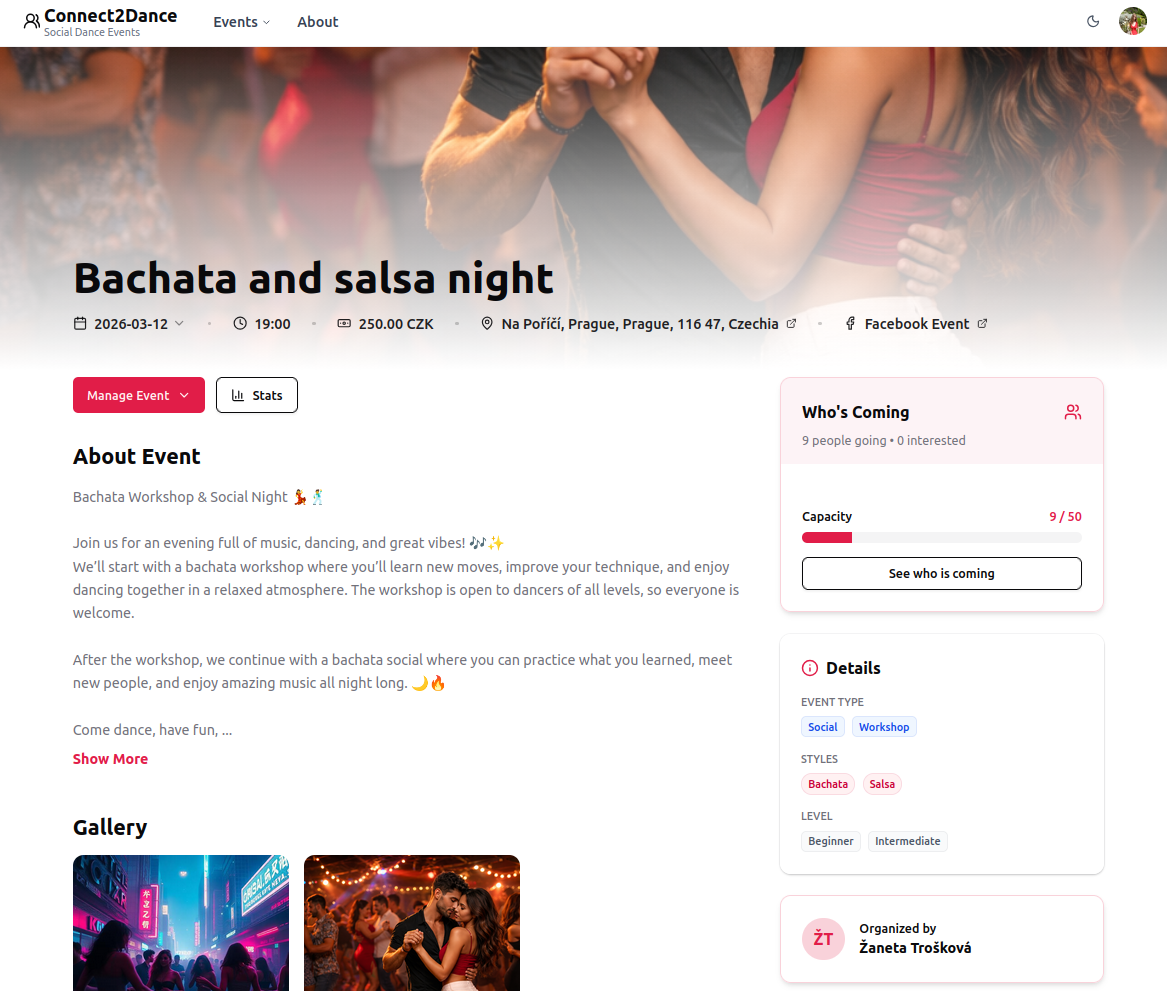
\includegraphics[width=\textwidth]{images/event-detail.png}
    \caption{Finální design detailu akce}
    \label{fig:eventDetail}
\end{figure}

\subsection{Modal na publikování akce}
Obvykle modály na jednoduché akce jako např. smazání události nejsou třeba speciálně navrhovat. V případě publikace akce se, ale jedná o modal obsahující formulář, ze kterého uživatel vybírá jak chce publikovat akci. Způsoby publikace akce jsou popsány v požadavku TODO. Proto jsem se rozhodla tento modal navrhnout, aby bylo jasné, jak bude vypadat a jak bude fungovat. Modal obsahuje název "Publish event", krátký popis toho, co zveřejnění akce znamená a co se stane po zveřejnění, a dále obsahuje formulář s možností výběru způsobu zveřejnění akce. Pro všechny druhy publikace akce existuje možnost zda uživatel chce potvrzovat jednotlivé registrace uživatelů či ne.

\subsection{Profil uživatele}
Profil uživatele jsem se snažila navrhnout tak, aby byl přehledný a obsahoval důležité informace o uživateli. Zároveň jsem chtěla aby designem evokoval profil na sociální síti, protože jsou uživatelé na takové rozhraní zvyklí a bude pro ně přirozené se v něm pohybovat. Profil uživatele se skládá z dvou částí:
\begin{itemize}
    \item karta s informacemi o uživateli, která obsahuje informace jako jméno a příjmení uživatele, hlavní role v tanci(leader, follower, role rotation), avatar uživatele, obecná úroveň v tanci, popis o sobě a taneční styly, které uživatel tancuje. Pokud je profil přihlášeného uživatele, tak se zde navíc nachází tlačítko pro úpravu profilu.
    \item galerie s obrázky a videi, které uživatel přidal do svého profilu. Galerie je řešena stejným designem jako u detailu akce.
\end{itemize}
Informace o tom co zobrazit v profilu uživatele jsem navrhla na základě požadavku TODO a galerii jsem navrhla na základě požadavku TODO.

Pokud jde o upravování profilu, tak po kliknutí na tlačítko pro úpravu profilu se zobrazí formulář, který umožní uživateli upravit informace na profilu. Sekce galerie se v v tomto případě přesune do karty s formulářem, kde uživatel může přidat nové obrázky a videa, nebo odstranit stávající.

Výsledný design profilu uživatele je znázorněn na obrázku \ref{fig:userProfile}.

\begin{figure}
    \centering
    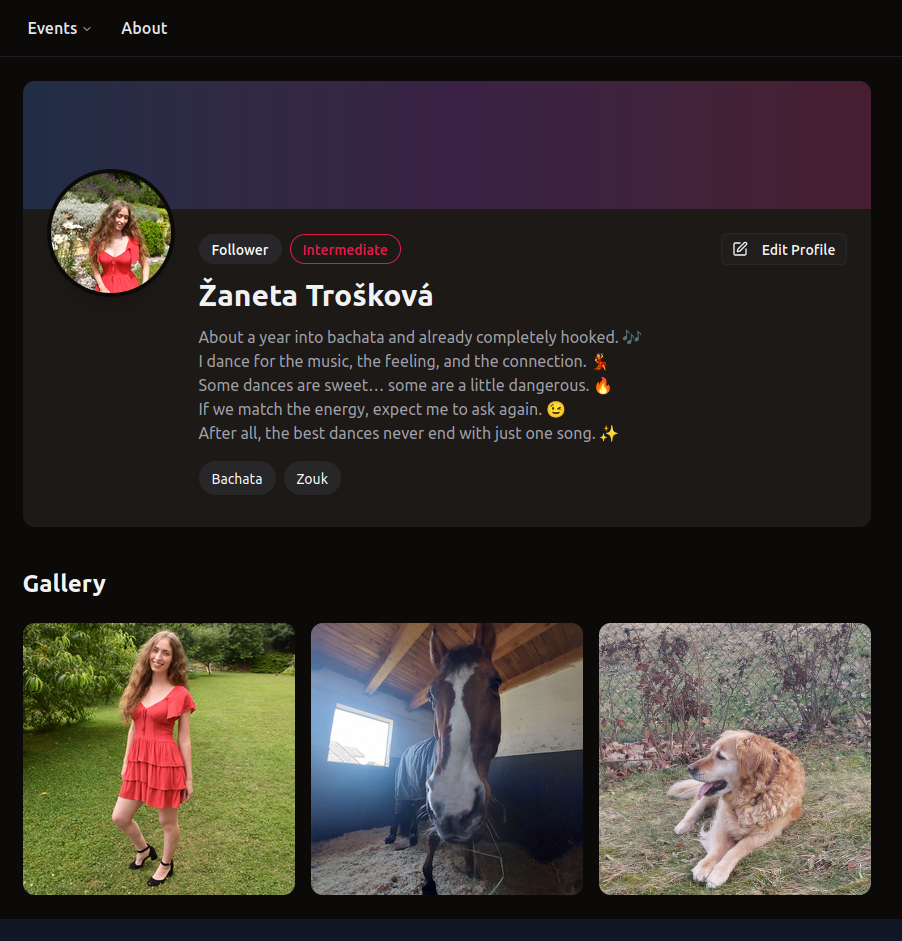
\includegraphics[width=\textwidth]{images/profile.png}
    \caption{Výsledný profil uživatele}
    \label{fig:userProfile}
\end{figure}

\subsection{Moje akce}
Tato stránka bude obsahovat seznamy akcí, které uživatel organizuje, na které se přihlásil a které označil že ho zajímají na základě požadavku TODO. Jelikož se jedná o seznamy, které jsou vzájemně disjunktní, navrhla jsem zobrazení pomocí komponenty Tabs, která umožní uživateli přepínat mezi jednotlivými seznamy. Zároveň se bude naho5e objevovat tlačítko pro vytvoření nové akce a nadpis "My events".

Pokud se jedná o akci, která je opakovaná, tak se zobrazí název celé této série s rozsahem datumů od první do poslední akce, a pod tím se zobrazí pomocí tabulky jednotlivé výskyty této akce. Tabulka obsahuje datum a čas konání výskytu, místo konání, počet přihlášených uživatelů a status akce, popřípadě status uživatele, pokud jsme v sekci přihlášených akcí. Také se pro každý výskyt nachází tlačítko pro zobrazení detailu výskytu, které přesměruje uživatele na detail výskytu akce. 

Pokud se jedná o akci, která není opakovaná, tak se zobrazí karta s názvem akce, datem a časem konání, místem konání, počtem přihlášených uživatelů a počtem uživatelů, kteří označili že je akce zajímá, a status akce, popřípadě status uživatele, pokud jsme v sekci přihlášených akcí. Také je zde tlačítko pro zobrazení detailu akce, které přesměruje uživatele na detail akce. 

Přemýšlela jsem nad tím, že minimálně v případě jednorázové akce bych nemusela implementovat tlačítko pro zobrazení detailu akce, ale místo toho by se uživatel mohl dostat na detail akce kliknutím na kartu s informacemi o akci. Nakonec jsem se však rozhodla implementovat tlačítko pro zobrazení detailu akce, protože mi přijde přehlednější a zároveň je to konzistentní s tím, jak je to v případě opakovaných akcí.

Pokud uživatel nemá žádné akce v dané sekci, tak se zobrazí karta s informací, že v této sekci nejsou žádné akce a s výzvou k tomu, aby uživatel začal procházet nadcházející akce a přihlásil se na nějakou z nich, nebo začal organizovat vlastní akci.

Na obrázku \ref{fig:myEvents} je znázorněna finální implementace této stránky v sekci událostí, které uživatel organizuje. Obrázek ukazuje, jak se zobrazí opakovaná akce, která má více výskytů, a také zobrazení jednorázové akce.

\begin{figure}
    \centering
    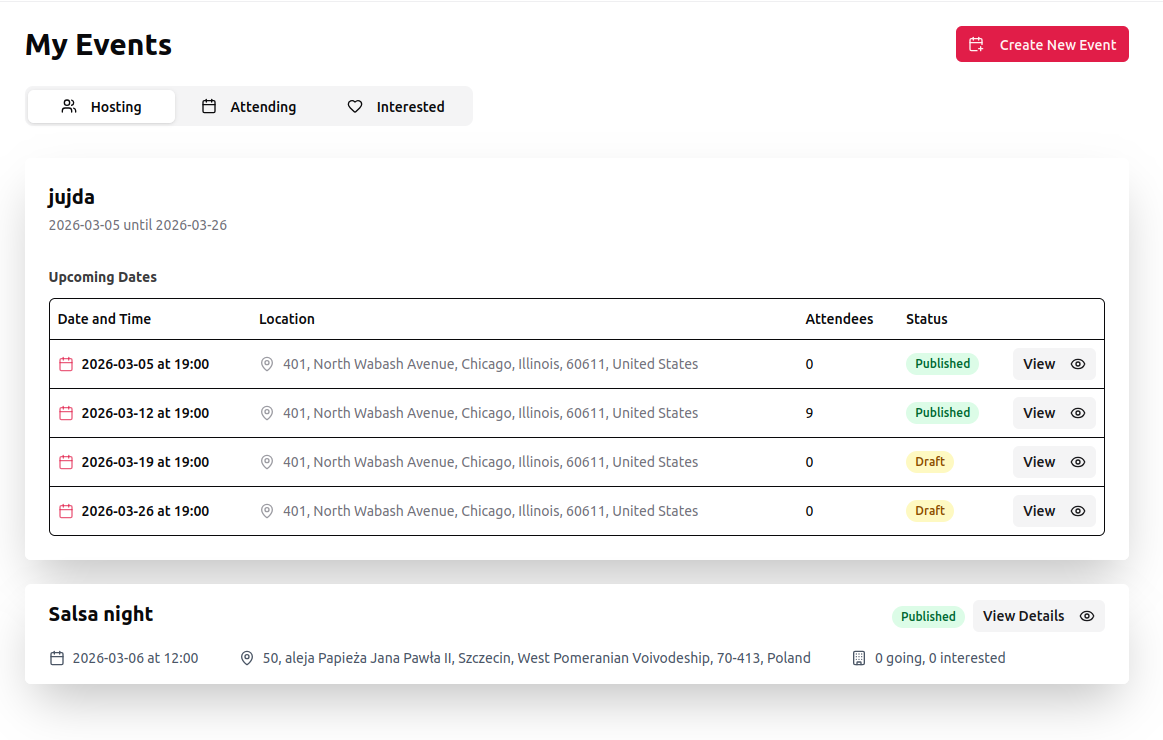
\includegraphics[width=\textwidth]{images/my-events.png}
    \caption{Finální implementace stránky "Moje akce"}
    \label{fig:myEvents}
\end{figure}

\subsection{Vytvořit akci}
Tuto část aplikace jsem navrhovala na základě požadavku TODO, který obsahuje informace o tom, jaké informace by měl formulář pro vytvoření akce obsahovat. 

Prvně jsem přemýšlela nad tím zda nemít jeden velký jednostránkový formulář. Toto řešení jsem navrhla protože z požadavku vyplívá, že pro vytvoření akce je potřeba zadat poměrně hodně informací, a já nechci aby se uživatelům zobrazoval příliš dlouhý formulář, který by je mohl odradit od vytvoření akce. Chvíli jsem ještě přemýšlela, že by sekce byly ve sbalitelných sekcích, což by mohlo napomoct k pocitu uživatele, že formulář není tak dlouhý. Avšak nakonec jsem se rozhodla rozdělit formulář do několika kroků, protože mi přijde přehlednější a mohu informace rozdělit do logických celků, což může uživatelům pomoci lépe se orientovat v tom, co mají zadat a zároveň se nemusí cítit zahlcení množstvím informací, které musí zadat najednou.

Existuje spousty způsobů, jak koncipovat aby každá sekce měla jednu stránku a mezi nimi se dalo přepínat. Pro inspiraci jsem procházela různé weby zaobírající se organizací akcí, jako například AllEvents. Na této stránce se používá pro přecházení mezi jednotlivými sekcemi formuláře boční nabídka. Toto řešení se mi moc nelíbí, protože mi přijde, že zbytečně zabírá místo na obrazovce a zároveň ve zbytku aplikace nepoužívám žádné boční menu, takže by to bylo nekonzistentní. 

Nakonec jsem se rozhodla pro řešení, které bude obsahovat kartu s jednotlivými kroky formuláře, která bude umístěna v levé části obrazovky a bude obsahovat název každého kroku a indikátor toho, který krok je aktuálně zobrazený. Po kliknutí na název kroku se uživatel přepne na tento krok. Toto řešení se mi líbí, protože je přehledné a uživatel je provázen celým procesem vytváření akce. Jediná nevýhoda tohoto řešení je, že zabírá místo na obrazovce, což na mobilních zařízeních může být problém. Proto jsem pro mobilní zobrazení navrhla, aby se místo karty s kroky zobrazoval pouze název aktuálního kroku a progres bar, který bude indikovat, kolik kroků uživatel již prošel a kolik jich ještě zbývá. V obou případech se budou tlačítka na přechod mezi jednotlivými kroky nacházet v dolní části obrazovky. Na posledním kroku se místo tlačítka pro přechod na další krok bude nacházet tlačítko pro odeslání formuláře a vytvoření akce.

Dalším krokem bylo jak rozdělit informace do jednotlivých kroků. Jelikož je informací poměrně hodně i v rámci jednoho kroku, tak jsem se snažila informace rozdělit do logických celků, které spolu souvisí.

Dospěla jsem k následujícímu rozdělení:
\begin{itemize}
    \item krok 1 - základní informace o akci
    \begin{itemize}
        \item základní informace o akci (jméno akce, lokace)
        \item datum a čas konání akce - v případě jednorázové lze navíc doplnit datum konce akce, v případě opakované akce datum posledního výskytu akce a frekvence opakování akce (denně, týdně, měsíčně)
        \item cena - kolik akce stojí a jaká je měna
    \end{itemize}
    \item krok 2 - popis akce - zvolila jsem proto tento prvek samostatný krok, protože z mých zkušeností bývá velmi dlouhý.
    \item krok 3 - média týkající se akce (zvolit primární obrázek akce, který se bude zobrazovat v přehledu nadcházejících akcí, a další obrázky a videa týkající se akce)
    \item krok 4 - doplňující informace o akci
    \begin{itemize}
        \item doplňující informace o akci (typ akce, typ tance, pro jakou úroveň tanečníků je akce určena, odkaz na facebookovou událost akce)
        \item informace ke kapacitě akce (maximální počet účastníků)
    \end{itemize}
\end{itemize}

\subsection{O aplikaci}
Tato stránka nebyla potřeba nijak vzlášť navrhovat, protože bude obsahovat pouze textové informace o aplikaci, které budou rozděleny do několika odstavců. 
Stránka bude obsahovat informace z požadavku TODO.

\subsection{Stránka s registrovanými uživateli}
Tato stránka bude přístupná pouze pro organizátory dané akce a bude obsahovat seznam všech registrací pro danou událost a možnosti s registrací pracovat (například zrušit registraci, přijmout registraci, atd.). 

Stránka bude tvořena názvem akce a pod ním bude datum akce. V případě že je akce opakovaná, bude zde stejná komponenta jako u detailu akce, která dovolí přepínat mezi jednotlivými výskyty akce.

Pod tím se bude nacházet tabulka, která bude obsahovat informace o registracích pro danou akci. Hlavička tabulky bude obsahovat zaškrtávací pole pro označení všech registrací, informace o uživateli, který se registroval, datum registrace a status registrace. 
Při zaškrtnutí konkrétní registrace se zobrazí možnosti pro práci s touto registrací, například zrušení registrace, přijetí registrace, atd. Každá hlavička tabulky obsahuje vhodný filtr pro každý sloupec, což může umožnit například filtrovat registrace podle statusu registrace, který organizátor chce vidět.

\subsection{Přihlašování a odhlašování z aplikace}
Pro přihlašování do aplikace jsem navrhla samostatnou stránku, která obsahuje kartu s tlačítkem umožňujícím přihlášení pomocí účtu Google. V případě potřeby rozšíření o další způsoby přihlašování, například pomocí e-mailu a hesla, by bylo možné tyto možnosti do stejné karty snadno doplnit.

Pokud se uživatel rozhodne z aplikace odhlásit, je po provedení této akce přesměrován na stránku s informací, že odhlášení proběhlo úspěšně. Tlačítko pro opětovné přihlášení jsem na tuto stránku záměrně neumísťovala, protože možnost přihlášení je již dostupná v navigační liště aplikace.








